\documentclass{article}
\usepackage[utf8]{inputenc}
\usepackage{cancel}
\usepackage{amsthm,amssymb,amsmath}
\usepackage{mathtools}
\usepackage{tikz}
% in preamble
\usepackage{movie15}
% in documenet

\usetikzlibrary{calc}
\usetikzlibrary{positioning}
\usepackage{parskip}
\usepackage{float}
\newtheorem{theorem}{Theorem}[section]
\newtheorem{corollary}{Corollary}[theorem]
\newtheorem{lemma}[theorem]{Lemma}
\setlength{\parskip}{1em}
\newcommand{\NN}{\mathbb{N}}
\newcommand{\ZZ}{\mathbb{Z}}
\newcommand{\RR}{\mathbb{R}}
\newcommand{\QQ}{\mathbb{Q}}
\newcommand{\CC}{\mathbb{C}}

\title{MAT 4800 Homework \# 4 }
\author{Noah Reef }
\date{Spring 2023}

\usepackage{natbib}
\usepackage{graphicx}

\begin{document}
\maketitle

\section*{Problem \#1}
\subsection*{Part a}
Suppose we are given the following function,

\begin{equation*}
    f(x_1,x_2) = 5x_1^2 + 2x_1x_2 + x_2^2 - x_1 + 2x_2 + 3
\end{equation*}

on $D = \RR^2$.

Here we will compute the Hessian as 

\begin{equation*}
    Hf = \begin{bmatrix*}
        10 & 2 \\
        2 & 2
    \end{bmatrix*}
\end{equation*}

by the principal minors approach we see that,
\begin{align*}
    \Delta_1 = 10 > 0 \\
    \Delta_2 = 20-4 = 16 > 0
\end{align*}

thus the Hessian is Positive Definite and thus $f(x_1,x_2)$ is convex, namely strictly convex by \textit{Theorem 2.3.7}.
\subsection*{Part b}
Suppose we are given the following function,

\begin{equation*}
    f(x_1,x_2) = \frac{x_1^2}{2} + \frac{3x_2^2}{2} + \sqrt{3}x_1x_2
\end{equation*}

on $D = \RR^2$.

\begin{equation*}
    Hf = \begin{bmatrix*}
        1 & \sqrt{3} \\
        \sqrt{3} & 3
    \end{bmatrix*}
\end{equation*}

by the principal minors approach we see that,
\begin{align*}
    \Delta_1 = 1 > 0 \\
    \Delta_2 = 0 
\end{align*}

thus the Hessian is Positive semi-definite and thus $f(x_1,x_2)$ is convex by \textit{Theorem 2.3.7}.

\subsection*{Part e}
Suppose we are given the following function,

\begin{equation*}
    f(x_1,x_2) = c_1x_1 + \frac{c_2}{x_1} +c_3x_2 + \frac{c_4}{x_2}
\end{equation*}

on $D = \{(x_1,x_2) \in \RR^2 : x_1 > 0, x_2 > 0\}$ where $c_i$ is a positive number for $i=1,2,3,4$.

\begin{equation*}
    Hf = \begin{bmatrix*}
        \frac{2c_2}{x_1^3} & 0 \\
        0 &  \frac{2c_4}{x_2^3}
    \end{bmatrix*}
\end{equation*}

by the principal minors approach we see that,
\begin{align*}
    \Delta_1 =  \frac{2c_2}{x_1^3} > 0 \\
    \Delta_2 = \frac{4c_2c_4}{x_1^3x_2^3} > 0
\end{align*}
thus the Hessian is Positive Definite and thus $f(x_1,x_2)$ is convex, namely strictly convex by \textit{Theorem 2.3.7}.

\section*{Problem \#2}
Suppose we have the function $f(\vec{x})$ defined on the set,
\begin{equation*}
    D = \{\vec{x} \in \RR^3: x_1 >0, x_2 > 0, x_3 > 0\}
\end{equation*}

by,

\begin{equation*}
    f(\vec{x}) = (x_1)^{r_1} + (x_2)^{r_2} + (x_2)^{r_2}
\end{equation*}
where $r_i > 0$ for $i = 1,2,3$

we compute the Hessian Matrix as,

\begin{equation*}
    Hf = \begin{bmatrix*}
        (r_1-1)r_1x_1^{r_1-2} & 0 & 0 \\
        0 & (r_2-1)r_2x_2^{r_2-2} & 0 \\
        0 & 0 & (r_3-1)r_3x_3^{r_3-2}
    \end{bmatrix*}
\end{equation*}
such that,

\begin{align*}
    d_1 &= (r_1-1)r_1x_1^{r_1-2} \\
    d_2 &= (r_2-1)r_2x_2^{r_2-2}\\
    d_3 &= (r_3-1)r_3x_3^{r_3-2}
\end{align*}

\subsection*{Part a}
Here if we assume that $r_i > 1$, then note by construction that
\begin{align*}
    d_1 &> 0 \\
    d_2 &> 0 \\
    d_3 &> 0 
\end{align*}

which means that the Hessian is \textbf{Positive Definite} and thus $f(x_1,x_2)$ is convex, namely strictly convex by \textit{Theorem 2.3.7}.

\subsection*{Part b}

Here if we instead assume that 
$r_i < 1$, then note by construction that
\begin{align*}
    d_1 &< 0 \\
    d_2 &< 0 \\
    d_3 &< 0 
\end{align*}

which means that the Hessian is \textbf{Negative Definite} and thus $f(x_1,x_2,x_3)$ is concave, namely strictly concave by \textit{Theorem 2.3.7}.

\section*{Problem \#3}

Suppose we are given the function,

\begin{equation*}
    f(x_1,x_2,x_3) = x_1^{-q}+x_2^{-r} + x_3^{-s}
\end{equation*}

defined on $D = \{(x_1,x_2,x_3) : x_1 > 0, x_2 > 0, x_3 > 0\}$ for $q,r,s \in \NN$. Here we first compute the Hessian matrix as,
\begin{equation*}
    Hf = \begin{bmatrix*}
        -(-q-1)qx_1^{-q-2} & 0 & 0 \\
        0 & -(-r-1)rx_2^{-r-2} & 0 \\
        0 & 0 & -(-s-1)sx_3^{-s-2}
    \end{bmatrix*}
\end{equation*}
such that,

\begin{align*}
    d_1 &=  -(-q-1)qx_1^{-q-2} = (q + 1)qx_1^{-q-2} > 0\\
    d_2 &= -(-r-1)rx_2^{-r-2} = (r+1)rx_2^{-r-2} > 0\\
    d_3 &= -(-s-1)sx_3^{-s-2} = (s + 1)sx_3^{-s-2} > 0
\end{align*}

Thus the Hessian is Positive Definite and thus $f(x_1,x_2,x_3)$ is convex, namely strictly convex by \textit{Theorem 2.3.7}.

\section*{Problem \#4}
Suppose we are given the following function,

\begin{equation*}
    f(x_1,x_2,x_3) = x_1\ln{x_1} + x_2\ln{x_2} + x_3\ln{x_3}
\end{equation*}
on $x_1,x_2,x_3 > 0$. Here we compute the Hessian as,
\begin{equation*}
    Hf = \begin{bmatrix*}
        \frac{1}{x} & 0 & 0 \\
        0 & \frac{1}{y} & 0 \\
        0 & 0 & \frac{1}{z}
    \end{bmatrix*}
\end{equation*}
such that,

\begin{align*}
    d_1 &=  \frac{1}{x} > 0\\
    d_2 &= \frac{1}{y}> 0\\
    d_3 &= \frac{1}{z} > 0
\end{align*}

Thus the Hessian is Positive Definite and thus $f(x_1,x_2,x_3)$ is convex, namely strictly convex by \textit{Theorem 2.3.7}.

\section*{Problem \#5}
Suppose we are given the function,

\begin{equation*}
    f(x_1,x_2) = \sqrt{x_1x_2}
\end{equation*}

with $x_1,x_2 > 0$. We compute the Hessian as,

\begin{equation*}
   Hf = \begin{bmatrix*}[r]
       
 -\frac{y^2}{4 (x y)^{3/2}} & \frac{1}{2 \sqrt{x y}}-\frac{x y}{4 (x y)^{3/2}} \\
 \frac{1}{2 \sqrt{x y}}-\frac{x y}{4 (x y)^{3/2}} & -\frac{x^2}{4 (x y)^{3/2}} \\
\end{bmatrix*}
\end{equation*}

Note that,

\begin{align*}
    \Delta_1 &= -\frac{y^2}{4 (x y)^{3/2}} < 0 \\
    \Delta_2 &= 0 
\end{align*}

Here we see that that the Hessian is Negative Semi-definite and thus $f(x_1,x_2,x_3)$ is concave by \textit{Theorem 2.3.7}. 
\section*{Problem \#6}
Suppose we are given the function,

\begin{equation*}
    f(x) = x + \frac{1}{x}
\end{equation*}

for $x > 0$. We first compute the derivative,

\begin{equation*}
    f'(x) = 1 - \frac{1}{x^2}
\end{equation*}

setting equal to $0$, we get

\begin{equation*}
    0 =  1-\frac{1}{x^2}
\end{equation*}
yields $x^*=1$ which is the critical point.

\subsection*{Part a}
By computing the second derivative we get

\begin{equation*}
    f''(x) = \frac{2}{x^3}
\end{equation*}

plugging in $x^*$ to get,

\begin{equation*}
    f''(1) = \frac{2}{1^3} = 2 > 0
\end{equation*}

Thus see that $x^*=1$ is a strict minimizer of $f(x)$.

\section*{Problem \#7}
Plotting the $f(x) = x + \frac{1}{x}$ we get,
\begin{figure}[H]
    \centering
    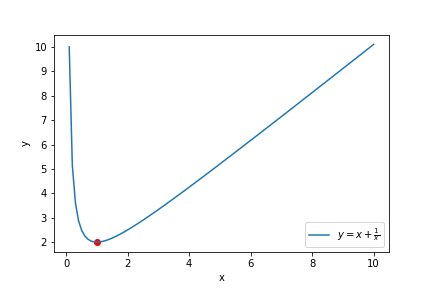
\includegraphics[scale=0.6]{graph1.png}
    \caption{Graph of $f(x) = x + \frac{1}{x}$}
    \label{fig:my_label}
\end{figure}

\section*{Problem \#8}
Suppose we are given,

\begin{equation*}
    g(x_1,x_2) = 2x_1^2 + x_2^2 + \frac{1}{2x_1^2 + x_2^2}
\end{equation*}

let $y(x_1,x_2)$ be defined as,

\begin{equation*}
    y(x_1,x_2) = 2x_1^2 + x_2^2
\end{equation*}
Computing the Hessian we get,

\begin{equation*}
   Hf = \begin{bmatrix*}[r]
       
4 & 0 \\
0 & 2
\end{bmatrix*}
\end{equation*}
which is Positive Definite and thus $y$ is convex.
we then rewrite $g$ as,

\begin{equation*}
    g(x_1,x_2) = f(y(x_1,x_2)) = y(x_1,x_2) + \frac{1}{y(x_1,x_2)}
\end{equation*}

note that from $(a)$the above equation has a global minimum at $y(x_1,x_2) = 1$, thus we find the critical points of $g$ lie on $2x_1^2+x_2^2 = 1$ which are the minimizers of $g(x_1,x_2)$, where $g(x_1,x_2) = 2$ by \textit{Theorem 2.3.10} since $y(x_1,x_2)$ is convex and $f(x)$ is increasing and hence $g(x_1,x_2)$ is convex.

\section*{Problem \#9}
\begin{figure}[H]
    \centering
    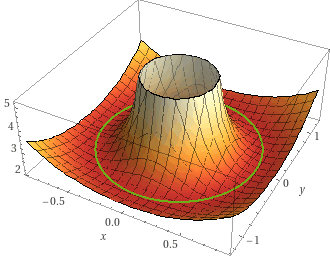
\includegraphics[scale=0.8]{download.png}
    \caption{graph of $g(x_1,x_2)$}
    \label{fig:my_label}
\end{figure}

\begin{figure}[H]
    \centering
    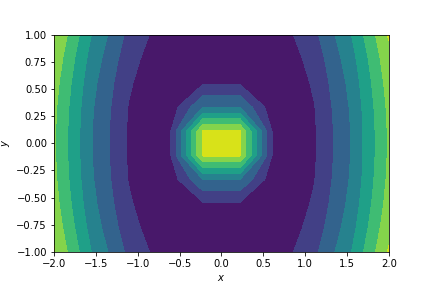
\includegraphics[scale=0.6]{graph3Contour (2).png}
    \caption{contour of $g(x_1,x_2)$}
    \label{fig:my_label}
\end{figure}
\section*{Problem \#10}
Suppose we are given,

\begin{equation*}
    h(x_1,x_2,x_3) = e^{x_1-x_2 + x_3}+ e^{-x_1 + x_2-x_3}
\end{equation*}

here we let $j(x_1,x_2)$ be defined as,

\begin{equation*}
    j(x_1,x_2,x_3) = x_1 - x_2 + x_3 
\end{equation*}

computing the Hessian as,

\begin{equation*}
   Hf = \begin{bmatrix*}[r]
       
0 & 0 & 0\\
0 & 0 & 0
\end{bmatrix*}
\end{equation*}
and is Positive Semi-definite, thus $j(x_1,x_2,x_3)$ is convex. Then we rewrite $h$ as,

\begin{equation*}
    h(x_1,x_2,x_3) = e^{j(x_1,x_2,x_3)}+ e^{-j(x_1,x_2,x_3)}
\end{equation*}

next let $t = e^{j(x_1,x_2,x_3)}$ to get,

\begin{equation*}
    h(x_1,x_2,x_3) = t + \frac{1}{t}
\end{equation*}

then we see that from $(a)$ we see that the minimizers occur at $t^* = 1$, thus we see,

\begin{equation*}
    e^{j(x_1,x_2,x_3) = 1
\end{equation*}

which implies that,

\begin{equation*}
    x_1 - x_2 + x_3 = 0
\end{equation*}

of which the plane defined above is the minimizers of $h$, with $h(x_1,x_2,x_3) = 2$,since $j(x_1,x_2,x_3)$ is convex and $f(x)$ is increasing and hence $h(x_1,x_2,x_3)$ is convex.
\end{document}